\documentclass[12pt, titlepage]{article}

\usepackage{booktabs}
\usepackage{tabularx}
\usepackage{hyperref}
\hypersetup{
    colorlinks,
    citecolor=black,
    filecolor=black,
    linkcolor=red,
    urlcolor=blue
}
\usepackage[round]{natbib}
\usepackage{graphicx}


%% Comments

\usepackage{color}

%\newif\ifcomments\commentstrue %displays comments
\newif\ifcomments\commentsfalse %so that comments do not display

\ifcomments
\newcommand{\authornote}[3]{\textcolor{#1}{[#3 ---#2]}}
\newcommand{\todo}[1]{\textcolor{red}{[TODO: #1]}}
\else
\newcommand{\authornote}[3]{}
\newcommand{\todo}[1]{}
\fi

\newcommand{\wss}[1]{\authornote{blue}{SS}{#1}} 
\newcommand{\plt}[1]{\authornote{magenta}{TPLT}{#1}} %For explanation of the template
\newcommand{\an}[1]{\authornote{cyan}{Author}{#1}}

%% Common Parts

\newcommand{\progname}{Inverted Pendulum Control Systems} % PUT YOUR PROGRAM NAME HERE
\newcommand{\authname}{Morteza Mirzaei} % AUTHOR NAMES                  

\usepackage{hyperref}
    \hypersetup{colorlinks=true, linkcolor=blue, citecolor=blue, filecolor=blue,
                urlcolor=blue, unicode=false}
    \urlstyle{same}
                                


\begin{document}

\title{Verification and Validation Report:\\ \progname \\ (IPCS)}
\author{\authname}
\date{\today}

\maketitle

\pagenumbering{roman}

\section{Revision History}

\begin{tabularx}{\textwidth}{p{3cm}p{2cm}X}
  \toprule {\bf Date} & {\bf Version} & {\bf Notes}      \\
  \midrule
  2024-04-13          & 1.0           & Initial Release. \\
  \bottomrule
\end{tabularx}

~\newpage

\section{Symbols, Abbreviations and Acronyms}

\renewcommand{\arraystretch}{1.2}
\begin{tabular}{l l}
  \toprule
  \textbf{symbol} & \textbf{description} \\
  \midrule
  T               & Test                 \\
  UT              & Unit Test            \\
  \bottomrule
\end{tabular}\\

\wss{symbols, abbreviations or acronyms -- you can reference the SRS tables if needed}

\newpage

\tableofcontents

\listoftables %if appropriate

\listoffigures %if appropriate

\newpage

\pagenumbering{arabic}

This document reports the results of executing the
\href{https://github.com/mirzaim/ipcs/blob/main/docs/VnVPlan/VnVPlan.pdf}{VnV Plan}.

\section{Functional Requirements Evaluation}
This section covers the evaluation of the functional requirements.

\subsection{test-input-1}
This test checks if the software returns proper exceptions for invalid inputs
and works properly for valid inputs. This test is implemented in
the file \url{https://github.com/mirzaim/ipcs/blob/main/test/test_integration.py},
and the function name is \texttt{test\_input\_1}. The test passed successfully.

\begin{small}
  \begin{verbatim}
test_integration.py::test_input_1[0.0-0.0--90.0-16.0-80.0-1.0-False]  PASSED
test_integration.py::test_input_1[abc-0.0--90.0-16.0-80.0-1.0-True]   PASSED 
test_integration.py::test_input_1[0.0-abc--90.0-16.0-80.0-1.0-True]   PASSED 
test_integration.py::test_input_1[0.0-0.0-abc-16.0-80.0-1.0-True]     PASSED   
test_integration.py::test_input_1[0.0-0.0--90.0-abc-80.0-1.0-True]    PASSED  
test_integration.py::test_input_1[0.0-0.0--90.0-16.0-abc-1.0-True]    PASSED  
test_integration.py::test_input_1[0.0-0.0--90.0-16.0-80.0-abc-True]   PASSED 
test_integration.py::test_input_1[0.0-0.0--90.0--16.0-80.0-1.0-True]  PASSED
test_integration.py::test_input_1[0.0-0.0--90.0-16.0--80.0-1.0-True]  PASSED
test_integration.py::test_input_1[0.0-0.0--90.0-16.0-80.0--1.0-True]  PASSED
test_integration.py::test_input_1[0.0-0.0--90.0-100.0-80.0-1.0-True]  PASSED
test_integration.py::test_input_1[0.0-0.0--90.0-16.0-100.0-1.0-True]  PASSED
test_integration.py::test_input_1[0.0-0.0--90.0-16.0-80.0-50.0-True]  PASSED
test_integration.py::test_input_1[0.0-0.0--90.0-5.0-80.0-1.0-True]    PASSED  
test_integration.py::test_input_1[0.0-0.0--90.0-90.0-80.0-1.0-True]   PASSED 
test_integration.py::test_input_1[0.0--20.0--90.0-16.0-80.0-1.0-True] PASSED
test_integration.py::test_input_1[0.0-20.0--90.0-16.0-80.0-1.0-True]  PASSED
  \end{verbatim}
\end{small}

\subsection{test-sim-1}
This section focuses on testing the world simulator responsible for
executing the inverted pendulum physics.
The testing procedure involves verifying that given the initial
position of the pendulum the location of the pendulum is accurately
determined after a specified duration of time.
This test is implemented in
the file \url{https://github.com/mirzaim/ipcs/blob/main/test/test_integration.py},
and the function name is \texttt{test\_sim\_1}. If the relative error
between the expected and actual values is less than $5\%$, the test is considered
successful. All the test passed successfully.

\begin{small}
  \begin{verbatim}
test_integration.py::test_sim_1[0.0-0.0--90.0-16.0-80.0-1.0-5.0-0.25]   PASSED 
test_integration.py::test_sim_1[0.0--5.0--90.0-16.0-80.0-1.0-5.0--4.75] PASSED
test_integration.py::test_sim_1[0.0-5.0--90.0-16.0-80.0-1.0-5.0-5.25]   PASSED 
test_integration.py::test_sim_1[0.0-0.0-0.0-16.0-80.0-1.0-6.0-0.08]     PASSED   
test_integration.py::test_sim_1[0.0-0.0--45.0-16.0-80.0-1.0-2.5--0.3]   PASSED 
test_integration.py::test_sim_1[0.0-0.0--90.0-30.0-80.0-1.0-1.5-0.8]    PASSED  
test_integration.py::test_sim_1[0.0-0.0--90.0-16.0-50.0-1.0-1.45-1.3]   PASSED 
test_integration.py::test_sim_1[0.0-0.0--90.0-16.0-80.0-20.0-5.0-0.25]  PASSED
test_integration.py::test_sim_1[5.0-0.0--90.0-16.0-80.0-1.0-2.7-0.65]   PASSED 
test_integration.py::test_sim_1[-5.0-0.0--90.0-16.0-80.0-1.0-5.5-0.0]   PASSED
  \end{verbatim}
\end{small}

\subsection{test-control-1}
The testing procedure involves verifying that given the initial
position of the pendulum the control system can keeping the pendulum
upright for 10 seconds after 30 seconds.
The test is implemented in the file
\url{https://github.com/mirzaim/ipcs/blob/main/test/test_integration.py}
and the function name is \texttt{test\_control\_1}.
All the test passed successfully.

\begin{small}
  \begin{verbatim}
test_integration.py::test_control_1[0.0-0.0--90.0-16.0-80.0-1.0]  PASSED 
test_integration.py::test_control_1[0.0--5.0--90.0-16.0-80.0-1.0] PASSED
test_integration.py::test_control_1[0.0-5.0--90.0-16.0-80.0-1.0]  PASSED 
test_integration.py::test_control_1[0.0-0.0-0.0-16.0-80.0-1.0]    PASSED   
test_integration.py::test_control_1[0.0-0.0--45.0-16.0-80.0-1.0]  PASSED 
test_integration.py::test_control_1[0.0-0.0--90.0-30.0-80.0-1.0]  PASSED 
test_integration.py::test_control_1[0.0-0.0--90.0-16.0-50.0-1.0]  PASSED 
test_integration.py::test_control_1[0.0-0.0--90.0-16.0-80.0-20.0] PASSED
test_integration.py::test_control_1[5.0-0.0--90.0-16.0-80.0-1.0]  PASSED 
test_integration.py::test_control_1[-5.0-0.0--90.0-16.0-80.0-1.0] PASSED
  \end{verbatim}
\end{small}

\subsection{test-vis-1}
This test checks the correctness of the visualization. We took 4 screenshots
(\autoref{fig:test_vis_1_1}, \autoref{fig:test_vis_1_2}, \autoref{fig:test_vis_1_3},
and \autoref{fig:test_vis_1_4}) of the visualization with different inputs.
The correctness of the visualization is evaluated and all the test passed successfully.

\begin{figure}[h!]
  \begin{center}
    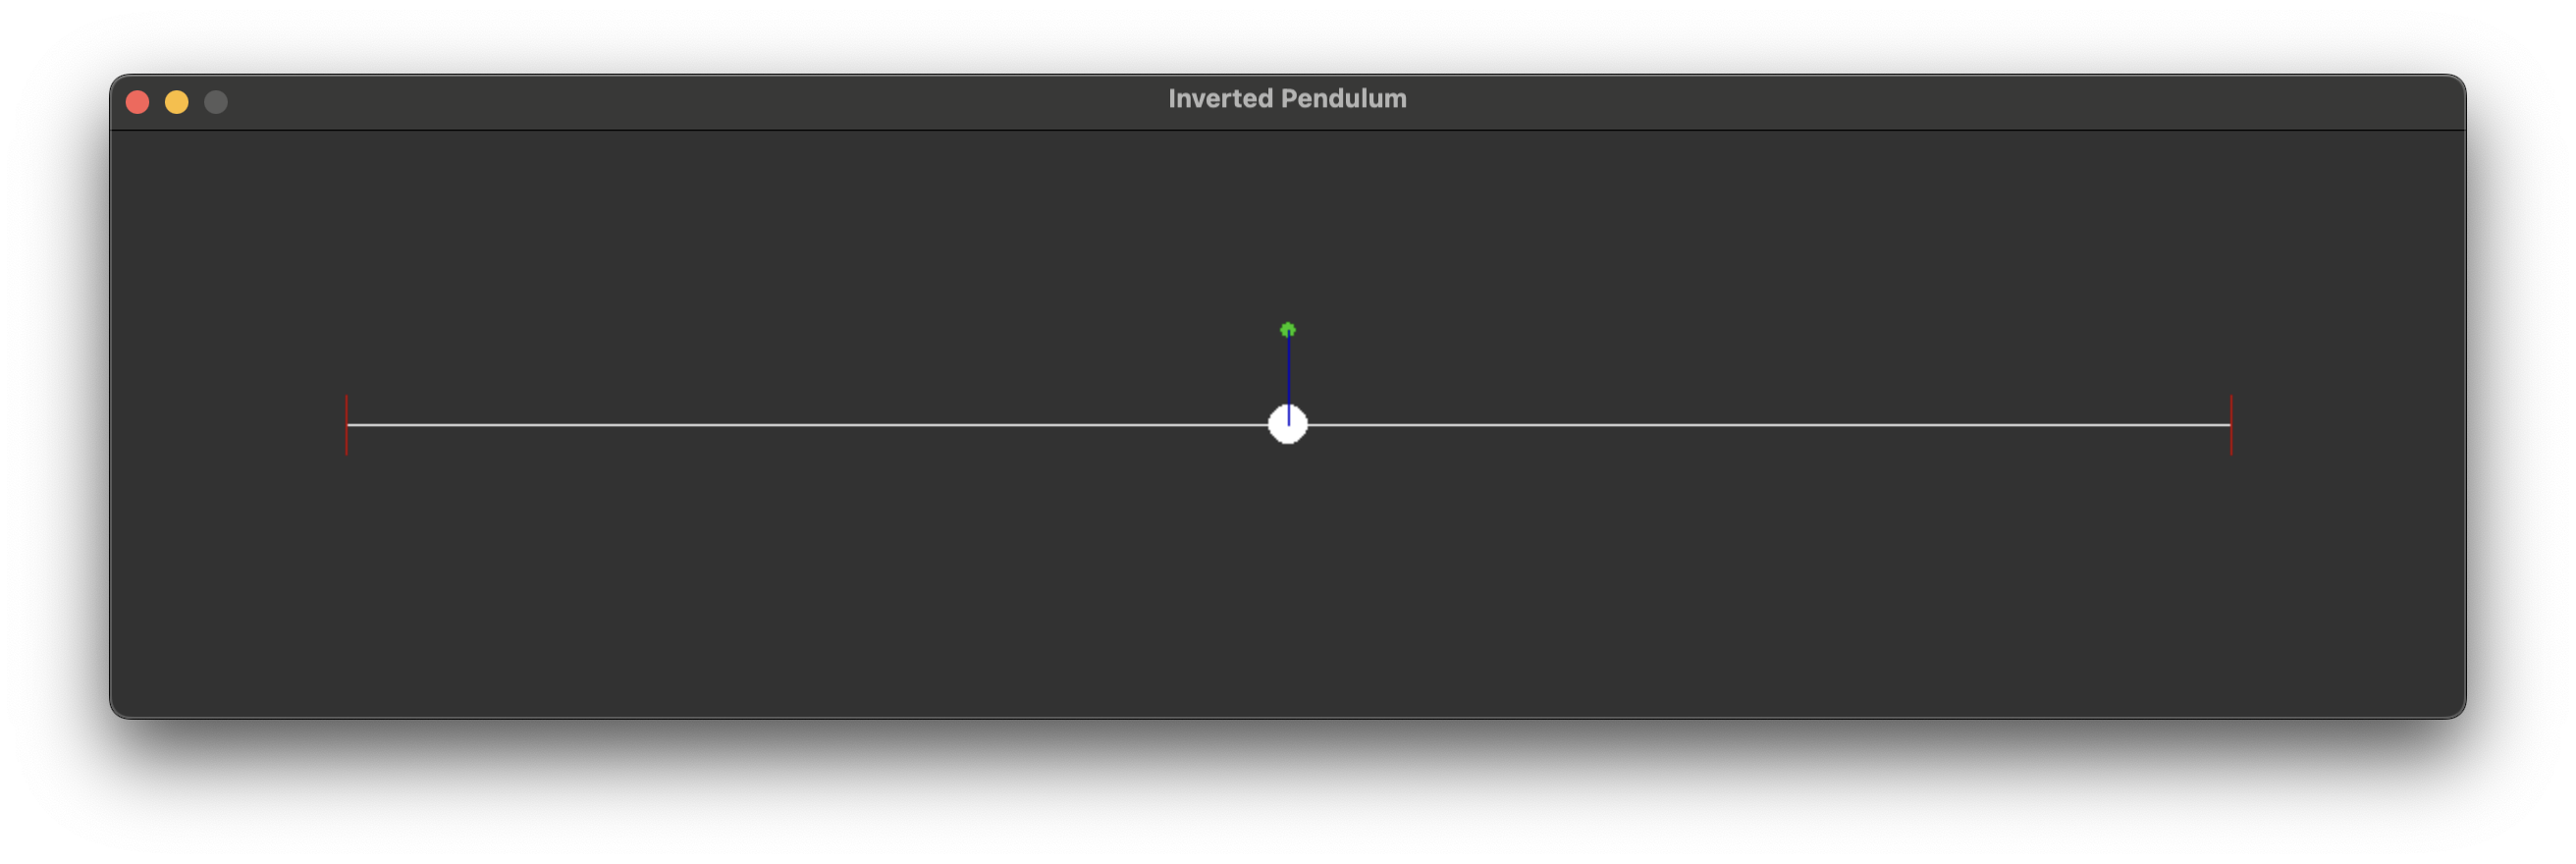
\includegraphics[width=\textwidth]{test_vis_1_1.png}
  \end{center}
  \caption{$x=0$ and $\theta=0$}
  \label{fig:test_vis_1_1}
\end{figure}

\begin{figure}[h!]
  \begin{center}
    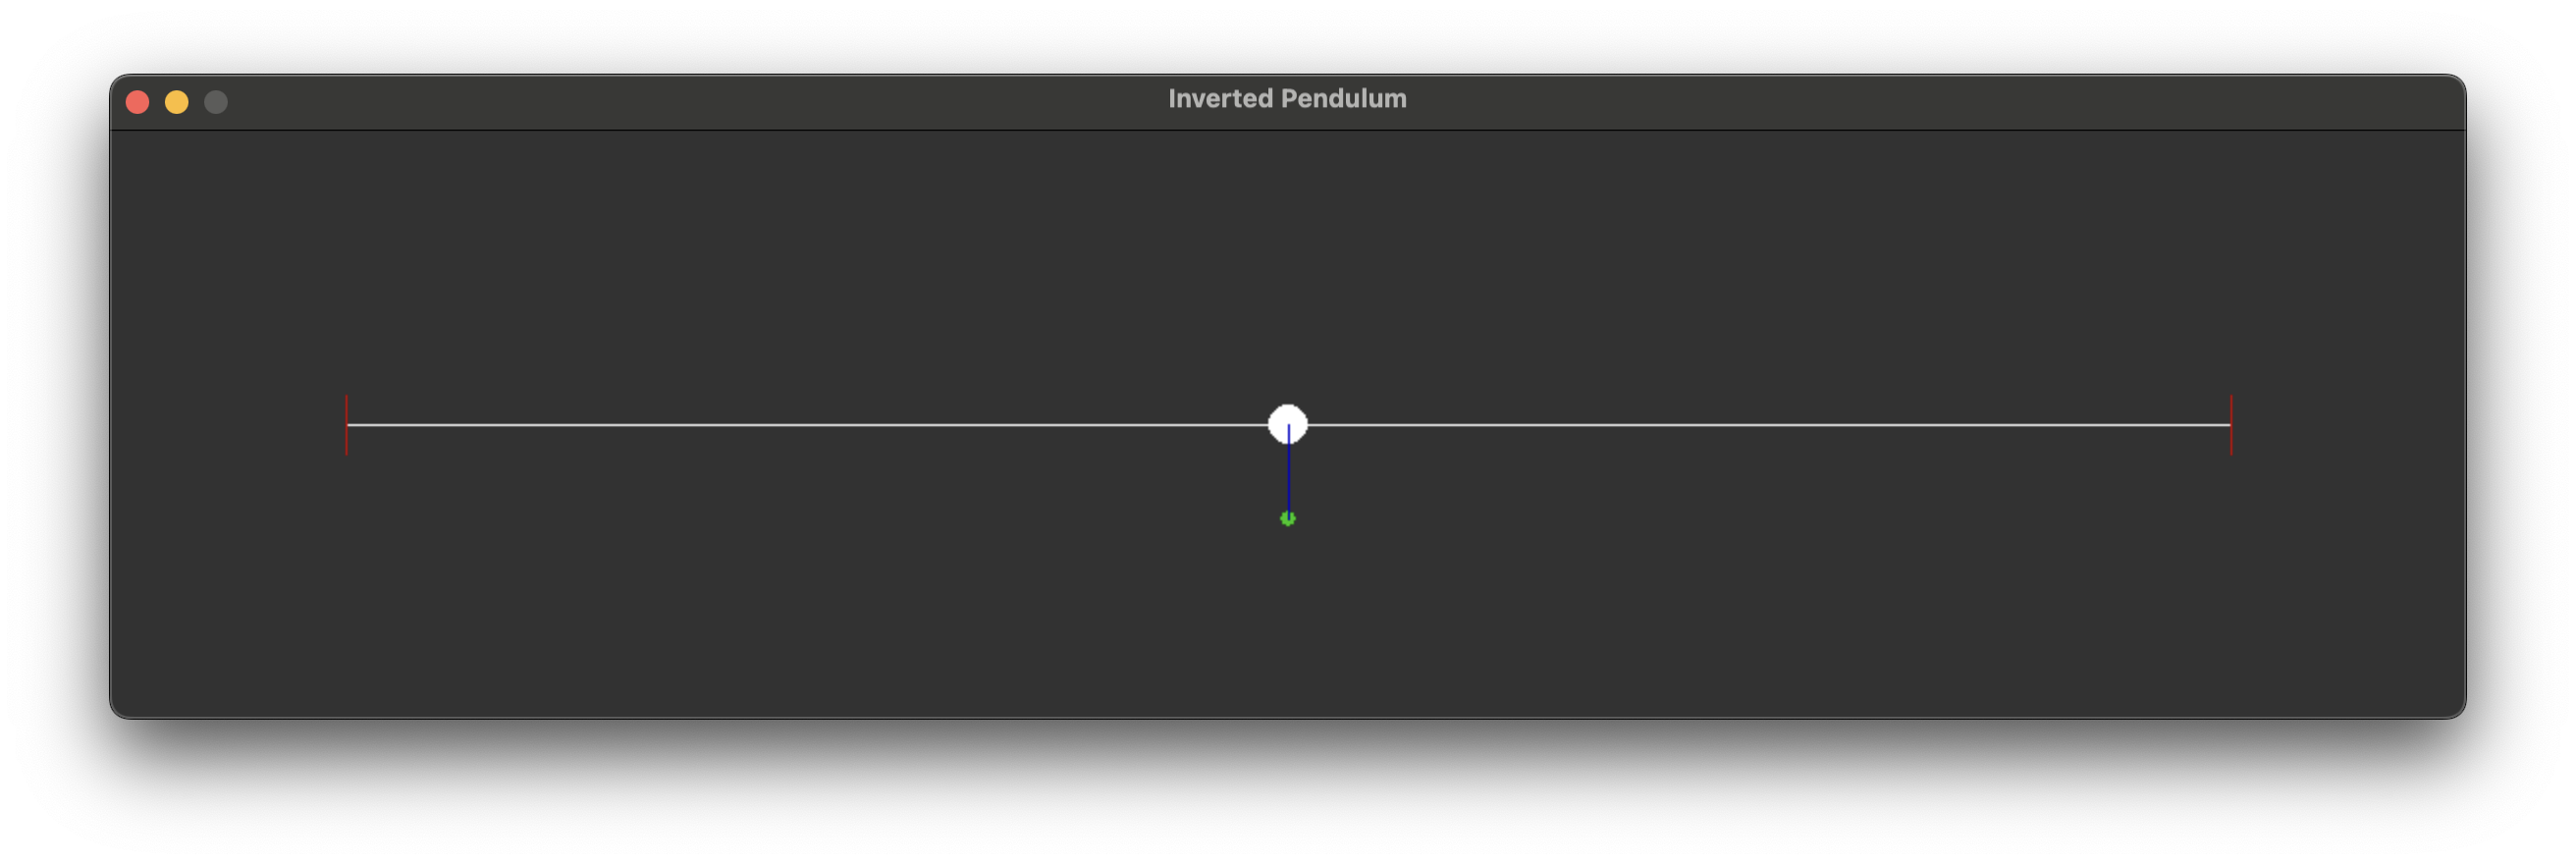
\includegraphics[width=\textwidth]{test_vis_1_2.png}
  \end{center}
  \caption{$x=0$ and $\theta=\pi$}
  \label{fig:test_vis_1_2}
\end{figure}

\begin{figure}[h!]
  \begin{center}
    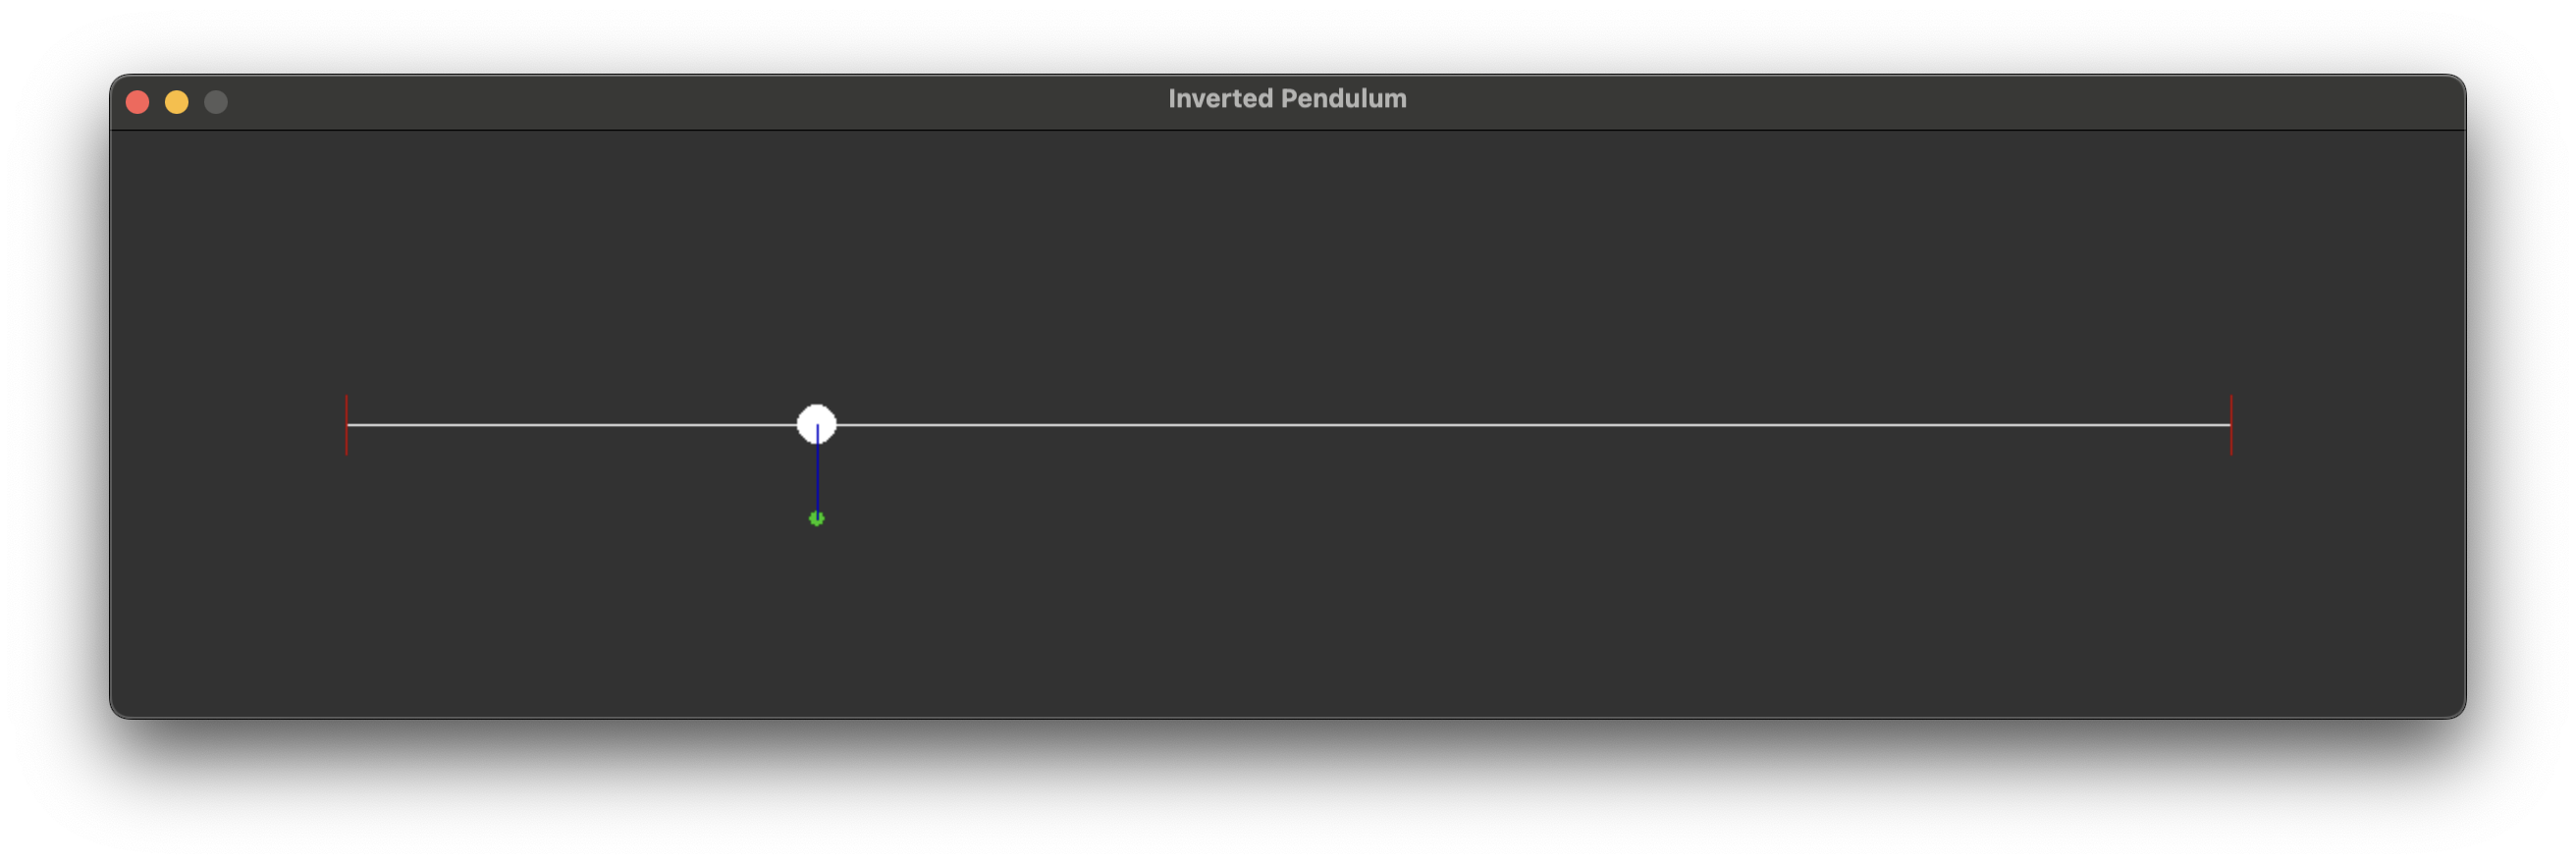
\includegraphics[width=\textwidth]{test_vis_1_3.png}
  \end{center}
  \caption{$x=-5$ and $\theta=\pi$}
  \label{fig:test_vis_1_3}
\end{figure}

\begin{figure}[h!]
  \begin{center}
    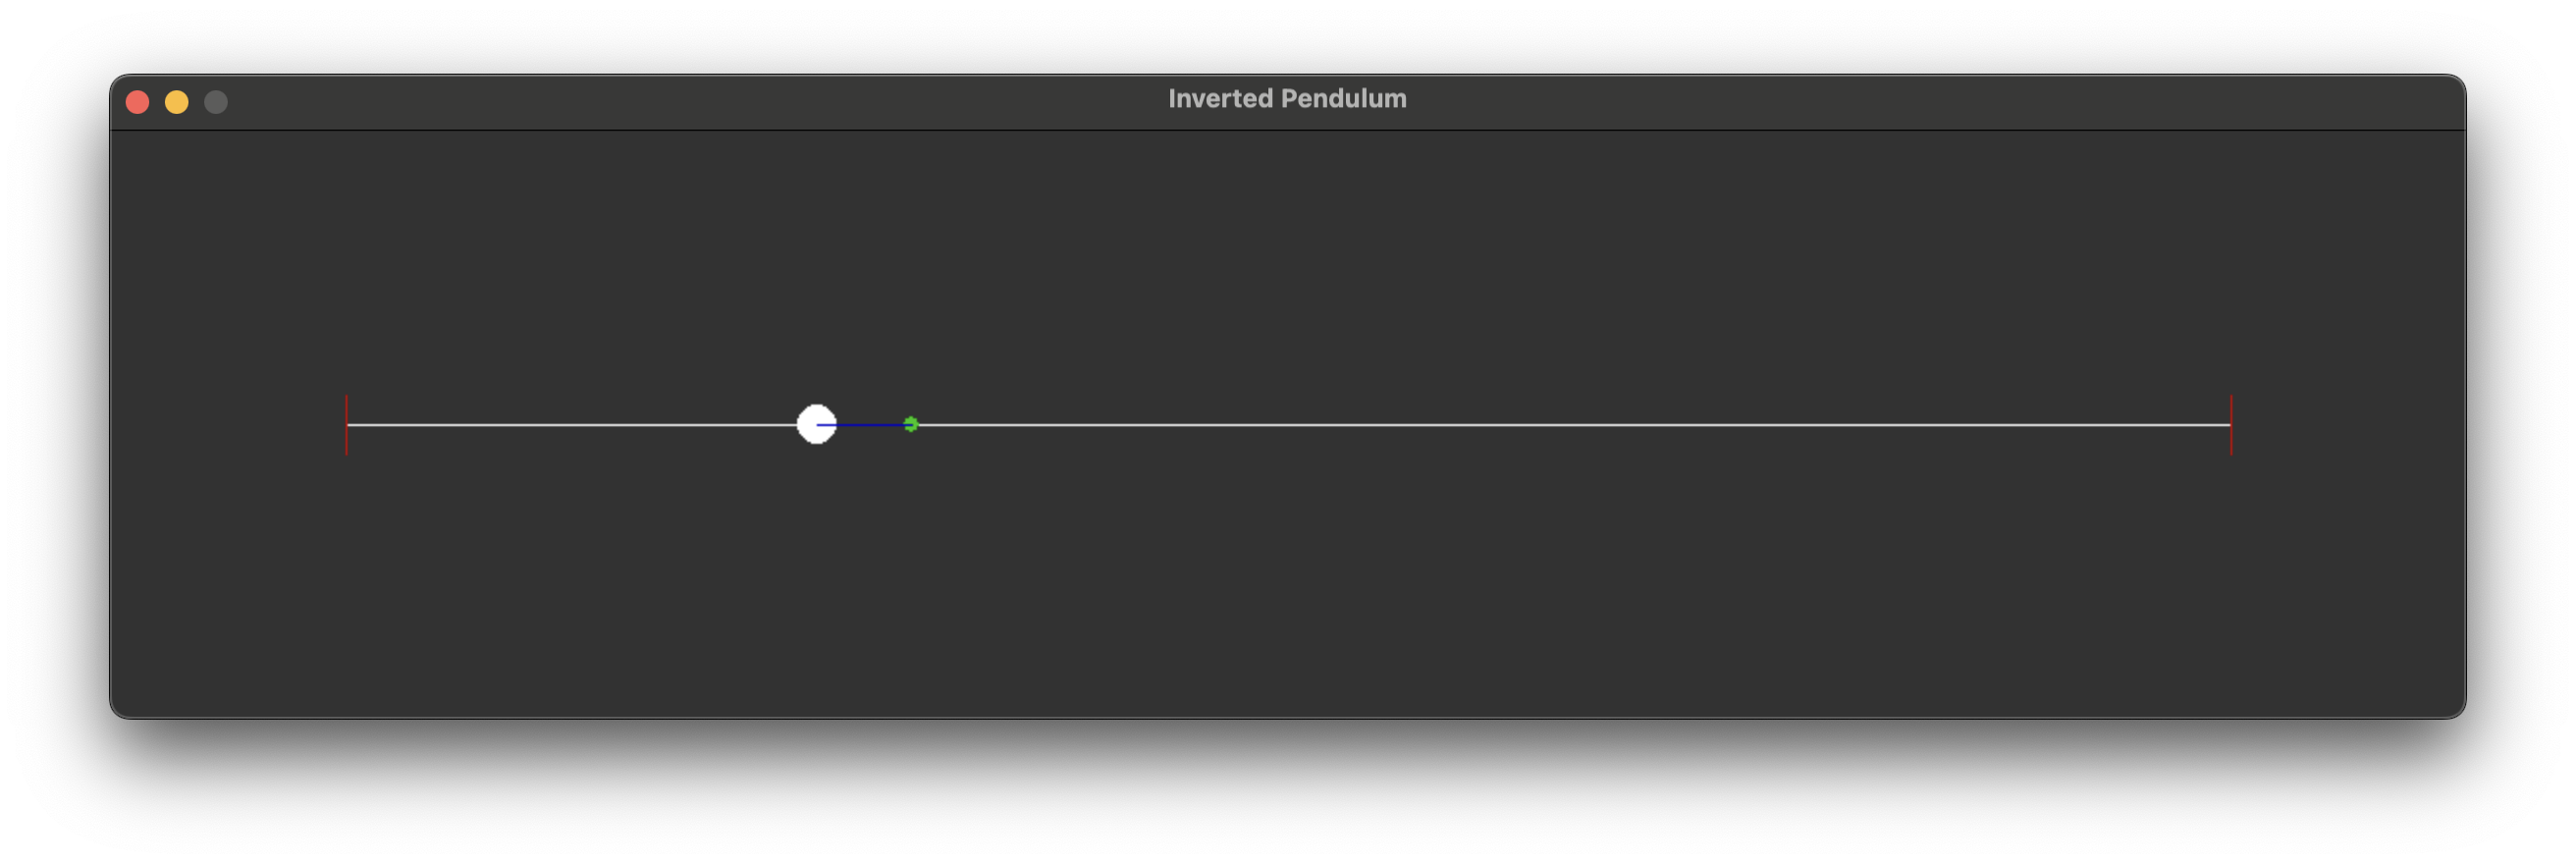
\includegraphics[width=\textwidth]{test_vis_1_4.png}
  \end{center}
  \caption{$x=-5$ and $\theta=\frac{\pi}{2}$}
  \label{fig:test_vis_1_4}
\end{figure}

\newpage

\subsection{test-vis-2}
This section focuses on testing the user-friendliness of the visualization aspect of the system.
The survey results conducted by the domain expert are shown in \autoref{tab:test_vis_2}.
The average score obtained is 4.75, which indicates a successful outcome.

\begin{table}[!h]
  \centering
  \caption{Domain expert feedback for test-vis-2. The average score is 4.75.}
  \label{tab:test_vis_2}
  \begin{tabular}{ p{0.5cm}|p{12cm}|c}
    \hline
    No. & Question                                                                        & Answer \\
    \hline
    1.  & On a scale of 1 to 5, how clear is the visualization to you?                    & 5      \\
    2.  & On a scale of 1 to 5, how clear is the location of the cart to you?             & 5      \\
    3.  & On a scale of 1 to 5, how clear is the angular position of the pendulum to you? & 5      \\
    4.  & On a scale of 1 to 5, how smooth is the visualization to you?                   & 4      \\
    \hline
  \end{tabular}
\end{table}

\section{Nonfunctional Requirements Evaluation}
This section covers the evaluation of the nonfunctional requirements.

\subsection{Accuracy}
The test is implemented in the file
\url{https://github.com/mirzaim/ipcs/blob/main/test/test_integration.py}
and the function name is \texttt{test\_acc\_1}.
The average relative error for cart location is $1.2\%$ and for pendulum angle is $2.4\%$.
The test passed successfully.

\subsection{Usability}
This section focuses on testing the usability of the system.
The survey results conducted by the domain expert are shown in \autoref{tab:useable}.
All the answers are positive, which indicates a successful outcome.

\begin{table}[!h]
  \centering
  \caption{Usability test survey, filled by the domain expert.}
  \label{tab:useable}
  \begin{tabular}{ p{0.5cm}|p{10cm}|c}
    \hline
    No. & Question                                             & Answer \\
    \hline
    1.  & Could you run the software on your operating system? & Yes    \\
    2.  & Is system running smoothly on your computer?         & Yes    \\
    3.  & Is invalid input's message clear?                    & Yes    \\
    4.  & Is text easy to read?                                & Yes    \\
    \hline
  \end{tabular}
\end{table}

\subsection{Maintainability}
This section is dedicated to assessing the system's maintainability.
The results of the survey, administered by a domain expert,
are presented in \autoref{tab:maintain}. All responses received were affirmative,
indicating a successful outcome.

\begin{table}[!h]
  \centering
  \caption{Maintainability test survey, filled by the domain expert.}
  \label{tab:maintain}
  \begin{tabular}{ p{0.5cm}|p{10cm}|c}
    \hline
    No. & Question                                                                                       & Answer \\
    \hline
    1.  & Does the design meet all specified requirements outlined in the design specification document? & Yes    \\
    2.  & Are all interfaces between design components specified clearly?                                & Yes    \\
    3.  & Are all components of the design testable separately?                                          & Yes    \\
    4.  & Is the design scalable to accommodate future growth or changes in requirements?                & Yes    \\
    5.  & Are the design components separated as much as possible?                                       & Yes    \\
    6.  & Does each design component have a logical task?                                                & Yes    \\
    \hline
  \end{tabular}
\end{table}

\subsection{Portability}
This section is dedicated to assessing the system's portability,
for which we conducted the following two tests.

\subsubsection*{test-port-1}
This test evaluates the system's portability across different operating systems,
specifically focusing on Linux and Mac OS.

\begin{enumerate}
  \item \textbf{Linux Testing:}
        The software is rigorously tested on Linux using GitHub workflows.
        After each push to the main branch, all tests are automatically
        executed on Ubuntu 22.04. The test results demonstrate
        successful execution.

  \item \textbf{Mac OS Testing:}
        Similarly, testing is conducted on Mac OS using a MacBook Pro 2022
        equipped with the M2 chip. All tests are executed on this platform,
        and once again, all tests pass successfully.
\end{enumerate}

\subsubsection*{test-port-2}
This test evaluates docker version of the software.
Every update to the main branch is automatically built and pushed to the
Docker Hub. The docker image is available at \url{https://hub.docker.com/r/mirzaim/ipcs}.
The docker image can be run using the following command:
\begin{small}
  \begin{verbatim}
sudo docker run -v ./out/:/ipcs/out --rm -it mirzaim/ipcs:latest
or
sudo docker run -v ./out/:/ipcs/out \
                -v <path to config file>:/ipcs/configs/default.ini \
                --rm -it mirzaim/ipcs:latest
  \end{verbatim}
\end{small}
The test passed successfully.

% \section{Comparison to Existing Implementation}

% This section will not be appropriate for every project.

\section{Unit Testing}

The files in the \url{https://github.com/mirzaim/ipcs/tree/main/test} directory
that starts with \texttt{test\_<module\_name>.py} are the unit tests.
We have 15 unit tests and 47 integration tests.
All the unit tests passed successfully.

\begin{small}
  \begin{verbatim}
test_checker.py::test_conf[conf0]                 PASSED                
test_checker.py::test_conf[conf1]                 PASSED                
test_checker.py::test_conf[conf2]                 PASSED                
test_conf.py::test_file_not_found                 PASSED                
test_conf.py::test_no_input_exception             PASSED            
test_fuzzy.py::test_fuzzy[world_conf0-0.0]        PASSED       
test_fuzzy.py::test_fuzzy[world_conf1-80.0]       PASSED      
test_fuzzy.py::test_fuzzy[world_conf2-0.0]        PASSED       
test_fuzzy.py::test_fuzzy[world_conf3-80.0]       PASSED      
test_simulator.py::test_exception[-1.0]           PASSED          
test_simulator.py::test_exception[-0.1]           PASSED          
test_simulator.py::test_exception[0.0]            PASSED           
test_simulator.py::test_tick[0.0-0.0-0.0-6.185]   PASSED  
test_simulator.py::test_tick[5.0-0.0-5.0-6.185]   PASSED  
test_simulator.py::test_tick[0.0--90.0-0.0-4.712] PASSED    
  \end{verbatim}
\end{small}

\section{Changes Due to Testing}

N/A.

\wss{This section should highlight how feedback from the users and from
  the supervisor (when one exists) shaped the final product.  In particular
  the feedback from the Rev 0 demo to the supervisor (or to potential users)
  should be highlighted.}

\section{Automated Testing}

The tests are set up to run automatically when a Pull Request is
opened and after any commit is made to the $\mathtt{main}$ branch.
The \href{https://github.com/mirzaim/ipcs/blob/main/.github/workflows/tests.yml}{GitHub workflow}
installs the required dependencies and runs the pytest command. Additionally,
after a successful pull request, the Docker image is built and pushed to the
\href{https://hub.docker.com/r/mirzaim/ipcs/tags}{Docker Hub}.

\section{Trace to Requirements}

The traceability between test cases and requirements is shown in \autoref{tab:traceability}.

\begin{table}[!h]
  \centering
  \caption{Relation of Test Cases and Requirements.}
  \label{tab:traceability}
  \begin{tabular}{|l|l|l|l|l|l|l|l|l|l|}
    \hline
                    & R1 & R2 & R3 & R4 & R5 & NFR1 & NFR2 & NFR3 & NFR4 \\ \hline
    test-inout-1    & X  &    &    &    &    &      &      &      &      \\ \hline
    test-sim-1      &    & X  & X  &    &    & X    &      &      &      \\ \hline
    test-control-1  &    &    &    & X  &    &      &      &      &      \\ \hline
    test-vis-1      &    &    &    &    & X  &      &      &      &      \\ \hline
    test-vis-2      &    &    &    &    & X  &      &      &      &      \\ \hline
    test-acc-1      &    & X  & X  &    &    & X    &      &      &      \\ \hline
    test-useable-1  &    &    &    &    & X  &      & X    &      &      \\ \hline
    test-maintain-1 &    &    &    &    &    &      &      & X    &      \\ \hline
    test-port-1     &    &    &    &    &    &      &      &      & X    \\ \hline
    test-port-2     &    &    &    &    &    &      &      &      & X    \\ \hline
  \end{tabular}
\end{table}

\section{Trace to Modules}

Traceability between test cases and modules is shown in \autoref{tab:traceability_modules}.

\begin{table}[!h]
  \centering
  \caption{Traceability Between Test Cases and Modules}
  \vspace{3mm}
  \label{tab:traceability_modules}
  \begin{tabular}{l|c}
    Module           & Tests    \\ \hline
    World Checker    & UT1      \\
    Config Reade     & UT2, UT3 \\
    Fuzzy Controller & UT4      \\
    Simulation       & UT5, UT6 \\
  \end{tabular}
\end{table}

\section{Code Coverage Metrics}

Code Coverage is out of scope of the VnV Plan.

% \bibliographystyle{plainnat}
% \bibliography{../References}

% \newpage{}
% \section*{Appendix --- Reflection}

% The information in this section will be used to evaluate the team members on the
% graduate attribute of Reflection.  Please answer the following question:

% \begin{enumerate}
%   \item In what ways was the Verification and Validation (VnV) Plan different
%         from the activities that were actually conducted for VnV?  If there were
%         differences, what changes required the modification in the plan?  Why did
%         these changes occur?  Would you be able to anticipate these changes in future
%         projects?  If there weren't any differences, how was your team able to clearly
%         predict a feasible amount of effort and the right tasks needed to build the
%         evidence that demonstrates the required quality?  (It is expected that most
%         teams will have had to deviate from their original VnV Plan.)
% \end{enumerate}

\end{document}